\section{Molecular Communication}
\subsection{Introduction}
\begin{itemize}
    \item Nano-machine (NM):
    \begin{itemize}
        \item[$\rightarrow$] nano-scale device able to perform a specific task at nano-level
        \item[$\rightarrow$] tasks done are simple $\rightarrow$ communicating, computing, data storing
        \item[$\rightarrow$] devices can be both articial and natural
        \item[$\rightarrow$] there are some similarities with cells:
        \begin{itemize}
            \item CPU $\rightarrow$ nucleus
            \item Power $\rightarrow$ mitochondrion
        \end{itemize}
        \item[$\rightarrow$] development approaches:
        \begin{itemize}
            \item Top-down $\rightarrow$ downscaling existing micro-scale level components
            \item Bottom-up $\rightarrow$ developed by using indivdual modules\\
            \hspace*{1.7cm}$\rightarrow$ not existing yet
            \item Bio-hybrid $\rightarrow$ biological nano-machines as models/building blocks\\
            \hspace*{2.1cm}to develop new nano-machines
        \end{itemize}
    \end{itemize}
    \item Nano-network $\rightarrow$ network of nano-machines
    \begin{itemize}
        \item[$\rightarrow$] it refers to electronic components
        \item[$\rightarrow$] components are interconnected with single chip on a nano-scale\\
        $\Rightarrow$ probably more biological than electronics
    \end{itemize} 
\end{itemize}
\subsection{Communication Media}
There are 3 types of communication:
\begin{itemize}
    \item Standard Communication
    \item Nano-mechanical Communication
    \item Molecular Communication
\end{itemize}
Here there is a detail description of all of them
\subsubsection{Standard Communication}
Characteristics:
\begin{itemize}
    \item it can be used:
    \begin{itemize}
        \item[$\rightarrow$] electromagnetic waves:
        \begin{itemize}
            \item given the size of NM, wiring a large quantity
            of them is unfeasible
            \item wireless solutions could be used $\rightarrow$ hard
            integration of antennas
            \item energy required to power the antenna is too high
        \end{itemize}
        \newpage
        \item[$\rightarrow$] acoustic waves:
        \begin{itemize}
            \item it needs transducers in NM $\rightarrow$ ability to sense waves
            \item size of transducers is very high
        \end{itemize}
    \end{itemize}
\end{itemize}
\subsubsection{Nano-mechanical Communication}
Characteristics:
\begin{itemize}
    \item information is transmitted through hard junctions
    between linked devices
    \item it requires physical contact between
    transmitter and receiver
\end{itemize}
\subsubsection{Molecular Communication}
Characteristics:
\begin{itemize}
    \item transmission and reception
    of information are encoded in molecules
    \item Most promising approach for nanonetworking:
    \begin{itemize}
        \item[$\rightarrow$] nolecular transceivers are already present at nano-level
        \item[$\rightarrow$] transmitters and receivers can be remotely located\\
        $\rightarrow$ as far as the transmitted molecules can go
    \end{itemize}
    \item there are 2 types of approaches:
    \begin{itemize}
        \item[$\rightarrow$] Short range communications:
        \begin{itemize}
            \item used for distances within mm
            \item Molecular motors:
            \begin{itemize}
                \item proteins $\Rightarrow$ transform
                chemical energy $\rightarrow$ mechanical work
                \item travel along molecular rails (microtubules), previously deployed
                \item data need to be encoded, transmitted and decoded
            \end{itemize}
            \item Calcium signalling:
            \begin{itemize}
                \item Responsible for many coordinated cellular tasks\\
                $\Rightarrow$ fertilization, contraction and secretion
                \item flexible $\rightarrow$ there is no need of railways
                \item similar to broadcast networks\\
                $\rightarrow$ all near nano-machines can receive a broadcast message
            \end{itemize} 
        \end{itemize}
        \item[$\rightarrow$] Long range communications
        \begin{itemize}
            \item used for distances from mm to km
            \item Pheromones:
            \begin{itemize}
                \item molecular compounds contains information\\
                $\rightarrow$ info only decoded by specific receivers
                \item messages consist of molecules $\Rightarrow$ a lot of different combination
                $\rightarrow$ in ants colony the whole communication is based on this
            \end{itemize}
            \item Bacteria:
            \begin{itemize}
                \item they have a number of interesting characteristics:
                \begin{enumerate}
                    \addtolength{\itemindent}{0.3cm}
                    \item[$\star$] Conjunction\\[0.15cm]
                    \hspace*{0.3cm}$\rightarrow$ it allows different bacterias to interconnect and pass\\
                    \hspace*{0.3cm}copies of plasmids (genetic messages)
                    \item[$\star$] Chemiotaxis\\[0.15cm]
                    \hspace*{0.3cm}$\rightarrow$ it is the movement induced into bacteria by chemica\\
                    \hspace*{0.3cm}stimuli:
                    \vspace*{-0.1cm}
                    \begin{enumerate}
                        \addtolength{\itemindent}{0.7cm}
                        \item[$\Rightarrow$] it swims towards food particles, like glucose
                        \item[$\Rightarrow$] it  swims away from poisons, like salts
                    \end{enumerate}
                    \hspace*{0.3cm}$\rightarrow$ they can communicate through simple emission of these\\
                    \hspace*{0.3cm}chemo-components
                    \item[$\star$] Resistance to antibiotics:\\[0.15cm]
                    \hspace*{0.3cm}$\rightarrow$ antibiotics filters/kills bacteria that don't contain\\
                    \hspace*{0.3cm}legitimate and/or complete plasmids\\[0.15cm]
                    \hspace*{0.3cm}$\rightarrow$ plasmids only gone through partial conjugation are\\
                    \hspace*{0.3cm}efficiently discarded
                \end{enumerate}
                \item Conjugation Based Opportunistic Routing
                \begin{enumerate}
                    \addtolength{\itemindent}{0.3cm}
                    \item[$\star$] opportunistic network is where:\\[0.15cm]
                    \hspace*{0.3cm}$\rightarrow$ contacts are intermittent\\[0.15cm]
                    \hspace*{0.3cm}$\rightarrow$ link performance is extremely variable
                    \item[$\star$] messages not intended for the recipients are dropped
                    \item[$\star$] chemoattractants are spread to achieve the wanted path
                    \item[$\star$] conjugation and chemotaxis are jointly used
                \end{enumerate}
            \end{itemize}
        \end{itemize}
    \end{itemize}
    \begin{figure}[!h] 
        \centering 
        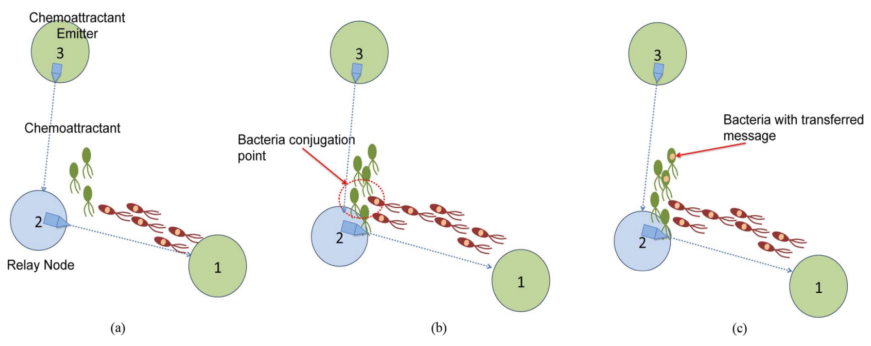
\includegraphics[scale = 0.39]{images/conjunction-routing.png} 
        \caption{Conjugation Based Opportunistic Routing}
        \label{conjunction-routing}
    \end{figure}
    \newpage
    \item Use Cases:
    \begin{itemize}
        \item[$\rightarrow$] Novel healthcare and medical technologies $\rightarrow$ live health monitoring
        \item[$\rightarrow$] Novel environment technologies $\rightarrow$ water resources monitoring
        \item[$\rightarrow$] Counter bioterrorism applications $\rightarrow$ referred to biological agents
    \end{itemize}
\end{itemize}
